\documentclass[portuguese]{textolivre}

% metadata
\journalname{Texto Livre}
\thevolume{18}
%\thenumber{1} % old template
\theyear{2025}
\receiveddate{\DTMdisplaydate{2024}{10}{25}{-1}}
\accepteddate{\DTMdisplaydate{2025}{2}{4}{-1}}
\publisheddate{\DTMdisplaydate{2025}{3}{22}{-1}}
\corrauthor{Gabriel Nicolau Souza}
\articledoi{10.1590/1983-3652.2025.55494}
%\articleid{NNNN} % if the article ID is not the last 5 numbers of its DOI, provide it using \articleid{} commmand 
% list of available sesscions in the journal: articles, dossier, reports, essays, reviews, interviews, editorial
\articlesessionname{articles}
\runningauthor{Nicolau de Souza e Silva}
%\editorname{Leonardo Araújo} % old template
\sectioneditorname{Daniervelin Pereira}
\layouteditorname{João Mesquita}

\title{Videoaulas e produção de artigo acadêmico: o que é ensinado?}
\othertitle{Videolessons and production of the academic article: what is taught?}

\author[1]{Gabriel Nicolau de Souza~\orcid{0009-0007-2591-6321}\thanks{Email: \href{mailto:gabrielnicolauestudante@gmail.com}{gabrielnicolauestudante@gmail.com}}}
\author[1]{Elizabeth Maria da Silva~\orcid{0000-0002-1355-493X}\thanks{Email: \href{mailto:elizabeth.maria@professor.ufcg.edu.br}{elizabeth.maria@professor.ufcg.edu.br}}}

\affil[1]{Universidade Federal de Campina Grande, Academia de Letras, Campina Grande, PB, Brasil.}


\addbibresource{article.bib}

%\usepackage{array,amssymb,calc,longtable,ulem}
\usepackage{longtable}

\usepackage{nameref}

%\makeatletter
%\let\orgdescriptionlabel\descriptionlabel
%\renewcommand*{\descriptionlabel}[1]{%
%  \let\orglabel\label
%  \let\label\@gobble
%  \phantomsection
%  \edef\@currentlabel{#1}%
%  %\edef\@currentlabelname{#1}%
%  \let\label\orglabel
%  \orgdescriptionlabel{#1}%
%}
%\makeatother

\makeatletter
\newcounter{descitem}
\let\orgdescriptionlabel\descriptionlabel
\renewcommand*{\descriptionlabel}[1]{%
  \let\orglabel\label
  \let\label\@gobble
  \phantomsection
  \refstepcounter{descitem}
  \edef\@currentlabel{\thedescitem}%
  \let\label\orglabel
  \orgdescriptionlabel{#1}%
}
\makeatother


\begin{document}
\maketitle
\begin{polyabstract}
\begin{abstract}
Neste trabalho, objetiva-se identificar e analisar
objetos de ensino explorados em videoaulas sobre produção de artigo
acadêmico. Metodologicamente, adota-se o método quanti-qualitativo, a
partir da netnografia. Como aporte teórico, apresentam-se práticas de
ensino de Língua Portuguesa em contexto didático-digital \cite{laurentino2023}, artigo acadêmico \cite{motta-roth2010}, as etapas de
produção textual \cite{antunes2003} e objetos de ensino \cite{linodearaujo2014}. Os dados constam de quinze videoaulas publicadas na plataforma
YouTube e destacam o foco na estrutura composicional do gênero como o
objeto de ensino mais recorrente. Observa-se que essa recorrência
decorre das especificidades do contexto didático-digital que abriga as
videoaulas, justificando seu modelo de produção e método de ensino.
Nesta análise, dá-se, assim, visibilidade a novos meios de ensino de
gêneros acadêmicos, como o artigo, e às formas pelas quais os objetos de
ensino são explorados em videoaulas.
 
\keywords{Contexto didático-digital \sep Videoaulas \sep Artigo
acadêmico \sep Objetos de ensino \sep Etapas de produção textual}
\end{abstract}

\begin{english}
\begin{abstract}
  This study aims to identify and analyze teaching
  components explored in videolessons about academic article production.
  Methodologically, the quantitative-qualitative method is adopted, based
  on netnography. As a theoretical contribution, Portuguese language
  teaching practices in a didactic-digital context are presented
  \cite{laurentino2023}, as well as academic article \cite{motta-roth2010}, stages of textual production \cite{antunes2003} and
  teaching components \cite{linodearaujo2014}. The data are contained in
  fifteen videolessons on the YouTube platform and highlight the focus on
  the compositional structure of the genre as the most recurrent teaching
  component. It is observed that this recurrence stems from the
  specificities of the didactic-digital context that houses the
  videolessons, justifying their production model and teaching method. In
  this analysis, visibility is thus given to new means of teaching
  academic genres, such as the article, and to the ways in which teaching
  components are explored in videolessons.
  
\keywords{Didactic-digital context \sep Videolessons \sep Academic
article \sep Teaching components \sep Stages of textual production}
\end{abstract}
\end{english}
\end{polyabstract}

\section{Introduction}\label{sec-intro}

Technology-assisted interpreting has experienced exponential growth in
recent years, reflected in the dizzying progress in the development of
information and communication technology (ICT) tools and resources
\cite{gutierrezArtacho2016,mezcua2019}. These innovative
technologies have greatly facilitated the interpretation and
comprehension of texts in different linguistic contexts \cite{olallaSoler2015}. In this sense, computer-assisted interpreting (CAI)
has become crucial in an increasingly globalised and connected society,
playing a pivotal role in breaking down language barriers and
facilitating effective communication in an environment characterised by
cultural and linguistic diversity \cite{mellinger2019,li2021}. In
response to the growing demand for instant online communication and the
need to overcome language limitations in a global environment, CAI has
established itself as an infallible tool for a wide range of
applications, from interpreting international business meetings to
translating multimedia content in real time \cite{fantinuoli2017a,alcaidemartinez2021}.

The integration of technology has revolutionised the way individuals
interact with language, opening new possibilities for increasing the
efficiency and accuracy of text interpretation, both in real time and
asynchronously \cite{gaber2023a,ramirezRodriguez2023}. The development
of ICT tools has led to improvements in natural language processing,
machine translation, speech recognition and other related technologies,
resulting in significant advances in text interpretation \cite{valeroGarces2024}. These tools have been particularly useful in overcoming language
barriers in multicultural environments, facilitating communication
between speakers of different languages and promoting intercultural
understanding \cite{perez2020}.

The use of CAI does, however, present certain difficulties. In the
phraseological domain, understanding idiomatic expressions remains a
significant challenge, as these linguistic constructions can be
particularly difficult to interpret accurately due to their cultural
embeddedness \cite{corpaspastorgaber2021,ramirezRodriguez2022}.
Cultural and contextual differences can lead to inaccurate or ambiguous
translations of these expressions, resulting in misunderstandings and
communication problems. In addition, CAI is often based on pre-defined
algorithms and databases, which can limit its ability to adapt to new
idioms and emerging expressions \cite{ortigoza2024}. This problem
identified in the interpretation of idiomatic expressions by CAI adds to
the previously mentioned challenges in technology-assisted phraseology,
where accuracy and fluency in the interpretation of texts in different
linguistic contexts are key to effective communication. The complexity
of idiomatic expressions, such as idioms, and their culturally
contextual nature require new approaches and specialised tools to
improve the interpretation of such expressions, which represents a
relevant area of research in the development of technology-assisted
phraseology.
\section{Embassamento Teórico}\label{sec-embasamento}

O referencial teórico utilizado como base norteadora deste estudo parte
do entendimento de contextos didático-digitais como um espaço advindo de
``publicações on-line de materiais com objetivo de conduzir sujeitos ao
domínio de saberes provenientes de disciplinas curriculares''
\cite[p.~46]{laurentino2023}. A partir dessa concepção, percebe-se
que a flexibilidade quanto ao modo de se ofertar conteúdos pedagógicos
atualmente, frente ao avanço tecnológico, potencializa um amplo alcance
e facilidade de acesso. Entretanto, essas vantagens não asseguram a
qualidade e a credibilidade dos conteúdos veiculados nesses contextos,
levando pesquisadores a examinarem criticamente a consistência desses
materiais \cite{bessa2020,laurentino_videoaulas_2019}.

A depender do material em questão, a forma como se estabelece o contato
entre usuário e conteúdo pode sofrer alterações. Em se tratando da
cibercultura, ambiente que abriga um acúmulo inquantificável de
conhecimento, ``o usuário pode interagir não só com o objeto (a máquina
ou a ferramenta), mas também com a informação, conteúdo'' \cite[p.~8]{rocha2005}. O modo de interação com o conteúdo se altera
conforme os componentes didáticos que complementam o material didático.
No caso da videoaula, a interação atinge o nível de mediação pedagógica
graças à sincronização de outras mídias (áudio, texto ou imagem)
\cite{barrere2014}, favorecendo a possibilidade de concretude dos fins
didáticos pretendidos.

Para considerarmos a videoaula um material didático-digital, \textcite{laurentino2023} apresentam outros componentes necessários para sua
caracterização, a saber: (a) tratar de uma prática de ensino que
apresente um foco didático, relacionando conhecimento curricular, teoria
e metodologia; (b) ser realizada de modo assíncrono; (c) apresentar a
figura de um sujeito empenhado em conduzir as práticas de ensino,
empregando saberes e competências relativos à profissão docente.

Com base nas informações supracitadas, podemos nos questionar: o que
justifica a alta demanda de acessos a materiais inseridos em contextos
didático-digitais? A resposta para essa pergunta pode se relacionar com
as ``práticas institucionais do mistério'', conforme estipulado por
\textcite{lillis1999}. O conceito explorado pela autora diz respeito a
convenções, sobretudo de escrita, demandadas aos alunos que não são
explicitamente orientadas, pois parte-se do pressuposto que eles já as
dominem. Em outras palavras, ``os professores esperam que os alunos
saibam essas convenções que não lhes são explicitadas'' \cite[p.~363]{fiad2011}. Esse cenário é comum na comunidade acadêmica, sobretudo por ser um
ambiente no qual são exigidas produções textuais específicas, típicas da
esfera acadêmica.

A alta demanda de produção de artigos acadêmicos advém da política de
financiamento de bolsas e de projetos de pesquisa, próprios do sistema
universitário brasileiro. Desse modo, nesse contexto, a produtividade
intelectual é medida pela produtividade na publicação \cite{motta-roth2010}. Esse fator gera uma pressão para elaboração de textos de
qualidade na forma de artigos para periódicos acadêmicos.

\textcite{motta-roth2010}, ao definirem o artigo acadêmico, já o
caracterizam como uma produção que objetiva a publicação em periódicos
especializados. Nas palavras das autoras, ``esse gênero serve como uma
via de comunicação entre pesquisadores, profissionais, professores e
alunos de graduação e pós-graduação'' \cite[p.~65]{motta-roth2010}. A exigência de produção de artigos acadêmicos pode se enquadrar em
uma ``prática institucional do mistério'' \cite{lillis1999}, caso suas
dimensões não sejam explicitadas aos produtores desse gênero. Essas
dimensões podem ser entendidas como: o enquadramento do gênero e do
público, contribuição para o avanço dos estudos de uma área de pesquisa,
a voz do autor e seu ponto de vista, as marcas linguísticas e sua
estrutura composicional \cite{street2010}. O aluno, ao se predispor a
produzir um artigo acadêmico, muitas vezes desconhece essas dimensões.

Não obstante defendamos a necessidade de apresentação aos estudantes de
orientações explícitas para as produções textuais, entendemos que a
finalidade pretendida não é de fornecer subsídios ou ``dicas'' de
produção, mas de permitir aos alunos ``uma produção do saber e
estabelecer uma base sólida para a construção contínua e eficaz de
conhecimentos específicos, desenvolvendo, ao mesmo tempo, a habilidade
de aprender e recriar permanentemente'' \cite[p.~48]{fischer2007}.

Ao abordar as habilidades ``de aprender e recriar permanentemente'', é
possível fazer um recorte das ponderações de \textcite{fischer2007} e refleti-lo
a partir de uma ótica textual. Mesmo que o artigo acadêmico traga
elementos constitutivos, em sua estrutura, como revisão da literatura,
metodologia, análise e discussão de resultados \cite{motta-roth2010}, há outras etapas inerentes à produção textual em si, exigidas
para uma prática constante de criação e recriação textual.

Elaborar um texto escrito é uma tarefa que não se completa pela
codificação de escrita e sintetização de ideias \cite{garcez2020}. Também
não se trata de uma atividade que se inicia quando tomamos nas mãos
papel e caneta ou quando nos ajustamos na cadeira com um documento
aberto e posicionamos as mãos no teclado. A escrita compreende três
etapas distintas e integradas de realização: planejamento, operação e
revisão \cite{antunes2003}. A autora compreende essas três etapas da
produção textual da seguinte forma: \emph{planejamento}: ``delimitar o
tema de seu texto e aquilo que lhe dará unidade, eleger os objetivos,
escolher o gênero, delimitar os critérios de ordenação das ideias,
prever as condições de seus leitores e a forma linguística (mais formal
ou menos formal) que seu texto deve assumir'' \cite[p.~55]{antunes2003};
\emph{operação}: registro do que foi planejado, escolha das palavras e
das estruturas das frases; \emph{revisão}: análise do que foi escrito,
para aquele que escreve confirmar o cumprimento dos objetivos, a
concentração temática desejada, a coesão e coerência no desenvolvimento
das ideias e se cumpriu com as normas gramaticais.

Podemos observar que apenas a atividade de escrita propriamente dita não
sustenta o processo de composição de uma produção textual. É necessária
uma etapa anterior e outra posterior, pois cada uma desempenha uma
função indispensável para produzir um texto que atenda seus objetivos de
produção.

Embora distintas, é importante alertar que as três etapas propostas por
\textcite{antunes2003} são intercomplementares. Ou seja, são etapas que implicam
umas nas outras e por isso, durante o ato de produção, não precisam ser
seguidas à risca, como se fossem métodos fixos e inflexíveis. ``Quando
planejamos, já estamos em plena escrita e, quando escrevemos, revisamos
simultaneamente parcelas do texto'' \cite[p. 20]{garcez2020}. O processo é
recursivo e, portanto, abre espaço para idas e vindas conforme
necessário.

Nessa perspectiva, esperamos que os materiais disponibilizados nos
contextos didático-digitais possam se comprometer com um ensino que
forneça essa base sólida de produção, advertindo ao público sobre as
etapas que precisam ser perpassadas ao escrever, para que possam
produzir o artigo acadêmico atentando-se aos seus próprios objetivos e
aos objetivos inerentes ao gênero trabalhado. Para tal, faz-se
necessário que o processo de ensino-aprendizagem sobre a produção desse
gênero em tela se estabeleça a partir de um ou mais objetos de ensino,
que orientem a metodologia empreendida para alcançar a finalidade
pretendida. \textcite[p.~11-12]{linodearaujo2014} apresenta três princípios
pelos quais são validados esses objetos, sendo eles:

\begin{quote}
Princípio da legitimidade -- o objeto precisa fazer referência aos
elementos que emanam da cultura ou são elaborados por especialistas;
Princípio de pertinência -- o objeto precisa estar relacionado às
capacidades dos alunos, às finalidades e objetivos da escola, aos
processos de ensino-aprendizagem; Princípio de solidarização -- objeto
precisa tornar coerentes os conhecimentos em função dos objetivos
visados.
\end{quote}

A seleção de objetos de ensino pode evidenciar, portanto, o modo como se
ensina determinado conteúdo. Para o estabelecimento de um objeto, é
preciso considerar o contexto de ensino e o conhecimento do público a
ser alcançado. A depender do caso, adaptações e reajustes são
necessários para que nenhuma informação passe despercebida pelos alunos.

Com base nessa compreensão de objetos de ensino, identificamos e, em
seguida, analisamos, na seção de resultados, quais objetos são
explorados em videoaulas sobre artigo acadêmico publicadas na plataforma
YouTube. Antes, apresentamos o método empreendido para selecionar as
videoaulas que constituem o \emph{corpus} da análise.

\section{Metodologia}\label{sec-metodologia}

Não foi necessária uma análise ética prévia por parte dos conselhos de
projetos adequados para a investigação, uma vez que os participantes não
foram identificados. Por não haver conflito de interesses, a Texto Livre
não terá quaisquer consequências, inclusive assistência integral e
eventual, ressarcimento de qualquer dano resultante a qualquer dos
participantes da pesquisa, conforme a Resolução nº 510, de 7 de abril de
2016, do Conselho Nacional de Saúde do Brasil.

A metodologia é a explicação minuciosa, detalhada, rigorosa e exata de
toda a ação desenvolvida no método de trabalho da pesquisa \cite{lakatos2003}. A pesquisa é um estudo de caso, que teve o aluno como
objeto de estudo. \textcite[p. 32]{yin2005} argumenta que o estudo de caso visa a \enquote{conhecer em profundidade o como e o porquê de uma determinada
	situação que se supõe ser única em muitos aspectos, procurando descobrir
	o que há nela de mais essencial e característico}. O estudo de caso é
caracterizado pelo estudo profundo e exaustivo de um ou poucos objetos,
de maneira a permitir o seu conhecimento amplo e detalhado. O caso
experimental caracteriza-se por determinar um objeto de estudo,
selecionar as variáveis que seriam capazes de influenciá-lo, definir as
formas de controle e de observação dos efeitos que a variável produz no
objeto \cite{gil2002}. A coleta dos dados foi realizada em uma escola
secundária do sul de Moçambique. Fizeram parte da amostra 50 alunos do
ensino secundário, selecionados de forma aleatória, dos quais 25
participaram do estudo das PO e aplicação do Q3DM. Os restantes 25
estiveram envolvidos no estudo das SCs e aplicação do GeoGebra. Em ambos
os estudos, todos os alunos experimentaram as aplicações (Q3DM ou
GeoGebra). A pesquisa apresenta um estudo de caso interpretativo, o qual
desenvolve categorias conceituais indutivamente para examinar os
pressupostos iniciais, as intenções e significados das ações e
expressões dos alunos \cite{amado2017}. A compreensão interpretativa é
sustentada a partir do relato pormenorizado da interação dos sujeitos em
seu meio natural \cite{coulon1995}. A visão interpretativa descreveu as
ações dos alunos em ambiente de sala de aula e os significados das ações
no processo de toda a pesquisa \cite{coutinho2011}.

Foi possível, pois, observar e interpretar tudo o que ocorreu, tornando
viável a análise das relações causa-efeito. Foi possível , também,
qualificar as ações dos alunos em todo o processo de aprendizagem, por
meio das interpretações dos significados de seus comportamentos durante
a mediação da aula e as respostas do questionário de satisfação. Além
disso, os dados foram coletados por meio das técnicas de observação do
participante, com tomada de notas e de registro fotográfico, assim como
dos instrumentos de coleta de dados aplicados, como os questionários de
satisfação.

\subsection{Realização das aulas}\label{sub-sec-Realização das aulas}

As aulas consistiram na apresentação de dois temas, PO e SCs, de forma
separada. Para os alunos da 9ª classe, o tema de pesquisa foi PO, e foi
utilizado o Q3DM. A professora primeiramente apresentou o tema,
explicando o que eram POs, dizendo que eram figuras geométricas sobre um
plano que poderiam ser comparadas à sombra do mesmo objeto no horário em
que o sol estaria no ponto mais alto no dia. Depois, demonstrou as
vistas ortogonais do sólido. (Ver \Cref{fig-03}).

\begin{figure}[htpb]
\centering
\begin{minipage}{.5\textwidth}
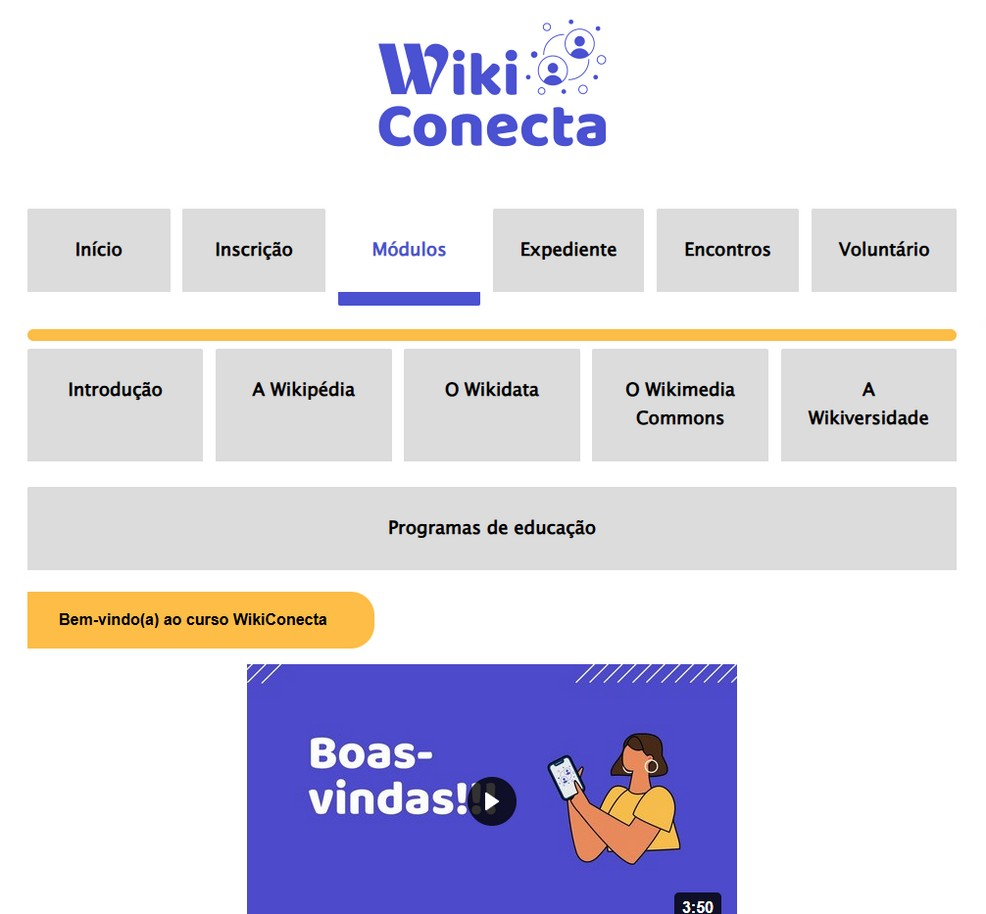
\includegraphics[width=\textwidth]{figures/figure03.jpg}
\caption{Vistas ortogonais e ortográficas: vista frontal; vista superior; e vista lateral esquerda.}
\label{fig-03}
\source{\url{http://turmag1215vialonga.blogspot.com/2014/10/projecoes-ortogonais.html}.}
\end{minipage}
\end{figure}

Posteriormente a professora apresentou a aplicabilidade das POs, dizendo
que eram destinadas à planificação de vários objetos. Com o auxílio das
simulações computacionais, construiu os sólidos geométricos e demonstrou
suas vistas ortogonais, apresentando os procedimentos para a manipulação
do Q3DM. (Ver \Cref{fig-04})

\begin{figure}[htpb]
\centering
\begin{minipage}{.5\textwidth}
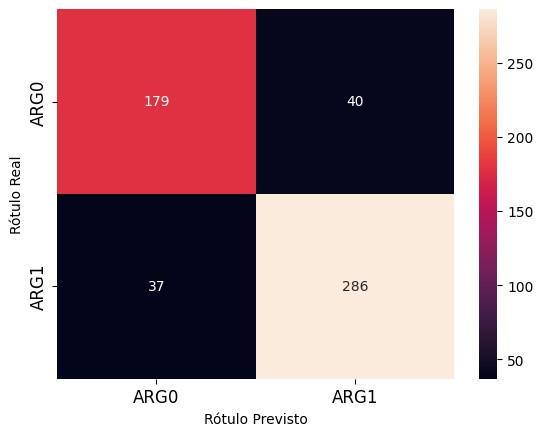
\includegraphics[width=\textwidth]{figures/figure04.jpg}
\caption{Manipulação no Q3DM.}
\label{fig-04}
\source{Elaboração própria.}	
\end{minipage}
\end{figure}


A manipulação no Q3DM é feita por meio de cubos chamados Qubes, que
facilitam a criação e a montagem de objetos em três dimensões,
utilizando elementos digitais que podem ser inseridos, removidos,
deslocados, ampliados, inclinados, moldados geometricamente, girados e
coloridos.

Para os alunos da 12ª classe, o tema de pesquisa foi SCs e foi utilizado
o GeoGebra. A professora iniciou com a apresentação do tema SCs de
cilindro, explicando que a seção cilíndrica é uma figura resultante de
um plano secante no cilindro. A professora acrescentou que existem duas
situações distintas: quando o plano secante é paralelo ao eixo central
do cilindro; e quando o plano secante não é paralelo ao eixo central do
cilindro (ver as figuras \Cref{fig-05} e \Cref{fig-06}).

\begin{figure}[htpb]
\centering
\begin{minipage}{.25\textwidth}
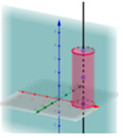
\includegraphics[width=\textwidth]{figures/figure05.jpg}
\caption{Secção paralela ao eixo central do cilindro.}
\label{fig-05}
\source{Elaboração própria.}
\end{minipage}
\end{figure}

\begin{figure}[htpb]
\centering
\begin{minipage}{.5\textwidth}
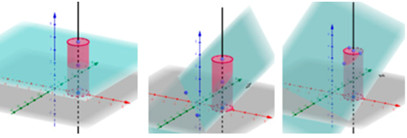
\includegraphics[width=\textwidth]{figures/figure06.jpg}
\caption{Secção não paralela ao eixo central do cilindro.}
\label{fig-06}
\source{Elaboração própria.}
\end{minipage}
\end{figure}

A professora, primeiramente, apresentou os diferentes posicionamentos
dos planos em relação ao eixo central do cilindro. Em seguida, com o
auxílio da tecnologia, apresentou à turma o software de geometria
dinâmica GeoGebra, indicando as funcionalidades de suas ferramentas e
como construir do ponto até o plano secante, com a ajuda dos
procedimentos para a sua manipulação no GeoGebra. Os alunos simularam as
SCs com o plano de nível; eles apresentaram-se atentos e motivados em
aprender a resolver o exercício no GeoGebra, particularmente para os
rapazes, os quais procuravam descobrir como construir diferentes sólidos
geométricos e como simular as VOs (vistas ortogonais).

\subsection{Realização do questionário}\label{sub-sec-Realização do questionário}

O questionário de satisfação aplicado teve como objetivo compreender se
o Q3DM e o GeoGebra facilitaram a aprendizagem das POs e SCs, e se o
\textit{smartphone} foi fácil de manipular. Ambos os questionários foram
preenchidos em 10 minutos. As questões visavam a coletar, nos dois
estudos, várias opiniões, incluindo: (1) se os aplicativos tecnológicos
facilitaram as representações 3D; (2) qual é a opinião deles sobre os
benefícios de usar os aplicativos ou se seria melhor resolver de forma
tradicional; (3) se os aplicativos são fáceis e intuitivos de usar; (4)
quais foram os aspectos positivos e negativos da aula; e, (5) como eles
classificariam a aprendizagem com o auxílio dos aplicativos.

\section{Objetos de ensino em videoaulas sobre artigo acadêmico}\label{sec-objetos}

Após o mapeamento das videoaulas listadas na \Cref{tab-01}, buscamos atender
aos dois objetivos deste trabalho: identificar e analisar objetos de
ensino explorados em videoaulas sobre artigo acadêmico publicadas na
plataforma YouTube.

Cabe destacarmos que, mesmo caracterizada por sua identidade assíncrona
e intermediada por um contexto didático-digital, entendemos que a
videoaula se firma como uma prática de ensino regida pelos três
elementos do sistema didático previstos por \textcite{linodearaujo2014}, a
saber: professor, aluno e ensino. O ensino, por sua vez, apenas será
concretizado se comprometido com as respostas à pergunta ``o que
ensinar?'', que, por conseguinte, respalda-se no ``como ensinar?''. Essa
linha de raciocínio nos conduz aos objetos de ensino, justamente por
serem ``construídos em processos nos quais saberes de referência são
transformados/adaptados para serem apresentados em {[}contexto{]} de
sala de aula'' \cite[p.~6]{linodearaujo2014}.

Ao transpormos essas proposições teóricas aos interesses da presente
pesquisa, notamos que os objetos de ensino explorados em videoaulas se
alinham de forma estrita ao contexto de produção e ao interesse do
público. Não se pode perder de vista que os materiais didático-digitais
são sustentados pela quantidade de acessos, pois esse fator influencia
na amplitude de acessos que as videoaulas podem receber. No processo de
construção analítica do presente trabalho, percebemos que o objeto de
ensino mais recorrente em todas as videoaulas é a estrutura
composicional do artigo acadêmico. Identificamos também outros objetos
de ensino: função do gênero, delimitação da pesquisa e etapas de
produção desse gênero (planejamento, operação e revisão). No caso dessas
etapas de produção, observamos que algumas tiveram maior visibilidade
que outras, havendo variação de uma videoaula para outra.

A partir dessa constatação sobre os objetos de ensino, organizamo-los da
seguinte forma: 4.1 Função do artigo acadêmico em videoaulas; 4.2
Estrutura composicional do artigo acadêmico em videoaulas; 4.3
Delimitação da pesquisa e 4.4 Etapas de produção textual.

\subsection{Função do artigo acadêmico em videoaulas}\label{sub-sec-funçãodoartigo}

Nesta seção, damos visibilidade a um dos objetos de ensino identificados
em algumas das videoaulas analisadas, a saber: a função do artigo
acadêmico. Vejamos a seguir três fragmentos extraídos de videoaulas
selecionadas, para exemplificar o modo pelo qual seus produtores
apresentam a função do artigo acadêmico:

\begin{description}
    \item[Fragmento 01\label{frag01}] -- Transcrição de conteúdo da videoaula 01 

    \begin{quote}
    /\ldots/ o artigo científico é o \textbf{menor trabalho acadêmico} em
termos de conteúdo. Ele é o que tem menor número de páginas, então a boa
notícia é\ldots{} você vai escrever\ldots{} menos. Além disso, os
artigos científicos são muito mais direcionados\ldots{} são muito mais
práticos\ldots{} têm um volume menor de conteúdo, mas são muito mais
objetivos\ldots{} isso é legal /\ldots/

    /\ldots/ Pra gente que tá no meio acadêmico \textbf{o artigo científico
serve pra dá notoriedade ao autor}. O que que é isso? Pra fazer o autor
ser reconhecido/\ldots/

    Disponível em: \url{https://www.youtube.com/watch?v=1ZWLlGtBJt0}. Acesso
em: 04 out. 2024. {[}grifo nosso{]}.
    \end{quote}

    \item[Fragmento 02\label{frag02}] -- Transcrição de conteúdo da videoaula 03

    \begin{quote}
    o artigo científico é \textbf{um tipo de trabalho acadêmico} que
apresenta resultados sucintos da sua pesquisa, utilizando métodos
científicos. \textbf{Algumas instituições de ensino, né\ldots{} algumas
faculdades\ldots{} elas exigem como forma de trabalho de conclusão de
curso} um artigo científico, tá?\ldots{} Então um trabalho de conclusão
de curso no formato de artigo científico /\ldots/.

    Disponível em: \url{https://www.youtube.com/watch?v=TnZroc6zey0\&t=93s}.
Acesso em: 04 out. 2024. {[}grifo nosso{]}.
    \end{quote}

    \item[Fragmento 03\label{frag03}] -- Transcrição de conteúdo da videoaula 14

    \begin{quote}
    /\ldots/ a verdade é que \textbf{pra você que faz mestrado ou doutorado,
muitas vezes, você precisa publicar esse artigo por uma exigência do seu
programa de pós-graduação}\ldots{} que só vai te dar um diploma de
mestrado ou doutorado, se você tiver um artigo publicado, né verdade?
/\ldots/

    Disponível em: \url{https://www.youtube.com/watch?v=omaqpo2b1JE}. Acesso
em: 04 out. 2024. {[}grifo nosso{]}.
    \end{quote}
\end{description}
 











Nos três fragmentos supracitados, os respectivos produtores das
videoaulas apresentam diferentes funções atribuídas ao artigo acadêmico
que justificam a sua produção escrita. Para \textcite[p.~66]{motta-roth2010}, essa função é atrelada à atividade de pesquisa, que subsidia
material para composição do artigo posteriormente, e ``está
essencialmente ligada ao meio universitário, onde professores e alunos
desenvolvem estudos avançados e pesquisas''. Na transcrição das
videoaulas, percebemos como de fato todos seus produtores consideram a
produção do artigo como uma atividade acadêmica, ao caracterizem o
gênero como ``\emph{o menor trabalho acadêmico}'' (Fragmento \ref{frag01}, linha
1) e ``\emph{um tipo de trabalho acadêmico}'' (Fragmento \ref{frag02}\hspace{0pt}, linha 1).

É perceptível na fala dos produtores de conteúdo que a produção do
artigo acadêmico é exigida tão somente para a obtenção de um diploma.
Nesse caso, a demanda desse gênero torna-se uma obrigação acadêmica que
desconsidera seus reais interlocutores e funções sociocomunicativas,
como por exemplo: compartilhamento de descobertas científicas entre os
pares, divulgação de conhecimentos construídos em pesquisas,
possibilidade de validação ou crítica por outros cientistas, entre
outros aspectos. No Fragmento \ref{frag02}, o produtor de conteúdo menciona que
``\emph{algumas faculdades\ldots{} elas exigem como forma de trabalho de
conclusão de curso um artigo científico}'' (linhas 3-4). Já no Fragmento \ref{frag03}, há um direcionamento para os alunos de pós-graduação: ``\emph{pra
você que faz mestrado ou doutorado, muitas vezes, você precisa publicar
esse artigo por uma exigência do seu programa de pós graduação}''
(linhas 1-2). Percebemos, portanto, que a produção de artigo acadêmico
tem sido uma demanda quase exclusiva a alunos de graduação e também de
pós-graduação. Não há menção a instruções por parte das instituições que
exigem a produção de tal gênero, de modo que os estudantes se veem
obrigados a produzi-lo, sem instrução prévia \cite{lillis1999} e/ou sem
estarem a par de um contexto sociocomunicativo que justifique sua
escrita e seu valor social.

Nos Fragmentos \hyperref[frag01]{1} e \hyperref[frag02]{2}, é possível observar que o público que os
produtores pretendem atingir são os graduandos. Ao citarem o Trabalho de
Conclusão de Curso (TCC), direcionam seu conteúdo àqueles encarregados
de produzir um artigo acadêmico para concluir sua graduação, atribuindo
sua função apenas como uma forma ``prática'' de se obter o diploma. O
Fragmento \ref{frag03}, no entanto, se direciona para os estudantes de
pós-graduação, para os quais, segundo a produtora, é exigida uma
produção constante também para obtenção de diploma. Um ponto de
convergência entre os Fragmentos \hyperref[frag01]{1} e \hyperref[frag03]{3} é a ``notoriedade'' citada pelo
primeiro. Essa notoriedade diz respeito aos profissionais que pretendem
seguir carreira no campo acadêmico, embora a menção tenha sido feita em
um tom pejorativo que estipula o artigo como uma mola propulsora para se
obter fama na comunidade acadêmica.

\subsection{Estrutura composicional do artigo acadêmico em videoaulas}\label{sub-sec-estrutura}


Na subseção anterior, vimos diferentes funções de artigo acadêmico, a
partir da transcrição das videoaulas de três produtores de conteúdo.
Ainda vimos como cada um atribui função ao gênero, e como a recorrência
é a de obrigatoriedade sobre a sua produção. No entanto, essas
constatações não sinalizam que toda área do conhecimento produz artigos
acadêmicos a partir de suas especificidades. Conforme afirmam \textcite[p.~66]{motta-roth2010}, ``cada área e cada problema de pesquisa
determinam o modo como a pesquisa será desenvolvida e, como
consequência, a configuração final do artigo que relatará a pesquisa''.
Ou seja, muito embora cada área aborde cada objeto de conhecimento a
partir de suas respectivas abordagens teóricas, os produtores de
conteúdo atendem às expectativas de um público geral e não-específico.
Por isso, muitos dos produtores recorrem ao ensino da estrutura e seus
aspectos constitutivos que resultam em uma abordagem da estrutura
composicional do gênero, que privilegia a forma como se constrói um
texto e quais as exigências que devem ser atendidas de acordo com o
contexto de circulação e com o público alvo. Conforme veremos a seguir
em outras transcrições selecionadas para ilustrar como é abordada a
estrutura composicional do artigo acadêmico nestas videoaulas:

\begin{description}
    \item[Fragmento 04\label{frag04}] -- Transcrição de conteúdo da videoaula 04

\begin{quote}
/\ldots/ \textbf{vamos falar sobre o que precisa ter num artigo\ldots{}
tá?\ldots{} os critérios básicos}. É claro que \textbf{num vídeo\ldots{}
só\ldots{} de\ldots{} de poucos minutos não é possível explorar todas as
possibilidades} de artigo dentro de uma metodologia. Então eu vou trazer
pra vocês o básico que precisa ter num artigo científico\ldots{} é,
quando eu falo básico, é a \textbf{estrutura básica} que tem que ter pra
que o texto é\ldots{} que você desenvolva, o estudo que você desenvolva
tenha aquela cara, aquele formato de científico /\ldots/.

Disponível em:
\url{https://www.youtube.com/watch?v=wzAXy7GEhSs\&t=431s}.
Acesso em: 04 out. 2024. {[}grifo nosso{]}.
\end{quote}

    \item[Fragmento 05\label{frag05}] -- Transcrição de conteúdo da videoaula 07

\begin{quote}
/\ldots/ as pessoas ficam dizendo por aí que TCC é difícil. Ora\ldots{}
qualquer tarefa é difícil pra quem não a conhece. Por isso eu resolvi
\textbf{fazer esse roteiro\ldots{} e te mostrar passo a passo de como
escrever um artigo científico}. \textbf{No meu curso, eu mostro em
detalhes cada uma das fases}\ldots{} de cada um desses passos. Por isso
meus alunos não sofrem\ldots{} apenas colocam em prática cada uma das
etapas\ldots{} na ordem que eu mostro sem depender de orientador\ldots.
\textbf{É claro que não dá pra mostrar tudo em apenas um vídeo pequeno
como esse}. Porém o mais importante que é o roteiro\ldots{} eu vou te
mostrar agora /\ldots/

Disponível em:
\url{https://www.youtube.com/watch?v=ZuojGmumuFY}.
Acesso em: 04 out. 2024. {[}grifo nosso{]}.
\end{quote}
\end{description}

Nos Fragmentos \hyperref[frag04]{4} e \hyperref[frag05]{5}, podemos observar a estrutura do gênero artigo
acadêmico como objeto de ensino referido nas respectivas videoaulas: na
04, ao propor abordar a ``\emph{estrutura básica}'' (\ref{frag04},
linhas 4-5) e na videoaula 07, ao mostrar o ``\emph{passo a passo de
como escrever um artigo científico}'' (Fragmento \ref{frag05}, linhas 2-3). Ao
considerarmos que o surgimento dos objetos de ensino se dá como produtos
de um processo de transposição didática \cite{linodearaujo2014}, e também
tendo em vista um público diverso advindo de áreas múltiplas, a
estrutura do artigo acadêmico se sobressai em detrimento de outros
objetos de ensino. Embora no Fragmento \ref{frag05} o produtor chame a estrutura
composicional do gênero de ``roteiro'', sua preocupação, assim como a do
produtor do Fragmento \ref{frag04}, é a de assinalar os movimentos retóricos
constitutivos do artigo acadêmico, a saber: introdução, revisão da
literatura, metodologia, análise e discussão dos resultados \cite{motta-roth2010}.

Não obstante a estrutura do artigo acadêmico como objeto de ensino, nas
referidas videoaulas, seja produtiva, não podemos desconsiderar as
especificidades disciplinares das áreas do conhecimento nas quais os
artigos são produzidos \cite{pereira2019}. As práticas de escrita
acadêmica, conforme destacam \cite{lea1998}, no âmbito da abordagem
dos letramentos acadêmicos, são plurais, situadas e heterogêneas.
Segundo esses autores, inclusive, não existe um único letramento
acadêmico, puro e homogêneo, mas, sim, letramentos acadêmicos, no
plural, marcados pelas relações específicas que estudantes, professores
e pesquisadores estabelecem com as práticas não só de escrita, mas
também de leitura, perpassadas por questões institucionais, de
identidade e autoridade. Todos esses aspectos não são evidenciados nas
videoaulas analisadas neste trabalho, algo preocupante, visto que quem
as assiste pode construir uma ideia equivocada de que só existe uma
forma de escrever artigo que pode ser aplicada em quaisquer contextos,
de acordo com a abordagem da socialização acadêmica \cite{lea1998}.

Ademais, não podemos desconsiderar a intenção mercadológica subjacente
às falas dos produtores de conteúdo que buscam apresentar uma
``amostra'' de cursos de produção escrita, como é possível notar nos
dizeres ``\emph{no meu curso, eu mostro em detalhes cada uma das
fases\ldots{} de cada um desses passos}'' (linhas 3-4) do Fragmento \ref{frag05}.
Essa intenção mercadológica não se restringe ao trecho transcrito, mas
se estende para tantos outros materiais, dado o alcance e a amplitude
que o contexto didático-digital proporciona.

Feita a identificação da estrutura do gênero, caminha-se para a
articulação das ideias que precisam constar em cada uma desses
constituintes. Entretanto, as ideias para produção de um artigo surgem
após o empreendimento de uma pesquisa. Vejamos como os produtores de
conteúdo abordam as delimitações de uma pesquisa que subsidiam a
produção do texto.

\subsection{Delimitação de pesquisa}

Conforme mencionado na subseção 4.1, o artigo acadêmico tem como função
materializar, em uma linguagem objetiva e concisa, os resultados de uma
pesquisa. Para a realização de uma pesquisa, é preciso elaborar o que é
conhecido como projeto de pesquisa que, segundo \textcite[p.~51—52, grifo das autoras]{motta-roth2010}, ``é uma das atividades humanas que
mais dependem de um planejamento prévio para que o(s) objetivo(s)
projetado(s) seja(m) alcançado(s). Comumente, o planejamento de uma
pesquisa é chamado de \emph{projeto}''. Ou seja, podemos notar que até
em outro gênero textual -- projeto de pesquisa --, o planejamento é uma
etapa vital. Entretanto, difere-se do que chamamos de ``planejamento
textual''.

Para a delimitação dos elementos constitutivos de um projeto de pesquisa
de mestrado, \textcite{silva2021} elenca como processo recursivo os seguintes
componentes: orientações teórico-metodológicas, sugestões do orientador,
ponderação: o que é pertinente e o que não é, sugestão da docente e dos
colegas. O autor caracteriza esses componentes como importantes e
não-lineares, ao passo que, ao ponderar sobre a delimitação de um
elemento, destaca ser necessário aplicar mudança em outros. Nas
videoaulas selecionadas, também encontramos a delimitação do projeto de
pesquisa como um objeto de ensino explorado, como podemos perceber no
fragmento a seguir:

\begin{description}
    \item[Fragmento 06\label{frag06}] -- Transcrição de conteúdo da videoaula 05

\begin{quote}
    /\ldots/ \textbf{a delimitação de um tema\ldots{} é a primeira etapa pra
que você\ldots{} comece a delimitação\ldots{} do seu objeto de
pesquisa}. Essa primeira etapa\ldots{} é fundamental pra que você
consiga \textbf{dar um rumo a sua pesquisa}\ldots{} e:: entender\ldots{}
\textbf{quais são seus objetivos}\ldots{} e onde você quer chegar nesta
pesquisa /\ldots/.

Disponível em:
\url{https://www.youtube.com/watch?v=bU_CMQvVtYE}.
Acesso em: 04 out. 2024. {[}grifo nosso{]}.
\end{quote}
\end{description}



No Fragmento \ref{frag06}, podemos observar como o produtor de conteúdo elenca a
delimitação do tema como a primeira etapa para compor o projeto de
pesquisa. Em suas palavras, ``\emph{essa primeira etapa é fundamental
pra que você consiga dar um rumo a sua pesquisa}'' (linhas 2-3). O rumo
ao qual ele se refere é a identificação dos objetivos, o que se pretende
alcançar com o empreendimento da pesquisa. Espera-se que os resultados,
alinhados ou não às expectativas do pesquisador, sejam reportados no
artigo acadêmico.

Tendo delimitado e realizado a pesquisa, a produção do artigo se
configura como o próximo passo. Assim como as demais produções textuais
escritas mais complexas, faz-se necessário atentar-se para as etapas que
constituem essa produção: planejamento, operação e revisão \cite{antunes2003}. Na próxima subseção, evidenciamos de que forma essas etapas de
produção textual são exploradas nas videoaulas analisadas.

\subsection{Etapas de produção textual} \label{sub-sec-etapas}


A estrutura não é o único ponto em comum para os estudiosos que
pretendem escrever um artigo acadêmico. As etapas de produção textual
\cite{antunes2003} são procedimentos inerentes a qualquer produção escrita,
logo poderiam ser consideradas tanto por aqueles que escrevem quanto por
quem ensina sobre escrita. Nessa perspectiva, ao analisarmos as
videoaulas em tela, observamos que seus produtores fazem, por vezes,
referência a tais etapas, conforme mapeamento que consta na \Cref{tab-02}:

{\footnotesize
\begin{longtable}{
    p{0.08\textwidth} 
    >{\raggedright\arraybackslash}p{0.27\textwidth} 
    >{\raggedright\arraybackslash}p{0.27\textwidth} 
    >{\raggedright\arraybackslash}p{0.27\textwidth}
}
    \caption{Etapas de produção textual mencionadas nas videoaulas sobre o ensino de produção de artigo acadêmico}\label{tab-02} \\
Videoaulas & Planejamento textual & Operação textual & Revisão textual \\
\midrule
\endhead
01/02\footnote{As videoaulas compostas por até dois vídeos distintos
  foram consideradas como um único material no momento da análise.
  Portanto, as videoaulas 01 e 02 foram analisadas de forma unitária,
  assim como as videoaulas 05 e 10.} & \checkmark

(roteiro que oriente a produção escrita) & \checkmark

(escrita após a conclusão do roteiro e identificação da estrutura) &
- \\
03 & - & - & - \\
04 & - & - & - \\
05/10 & - & - & - \\
06 & - & - & \checkmark

(adequação da linguagem e da pessoa do discurso) \\
07 & - & - & - \\
08 & \checkmark

(fluxo de ideia antes da produção, tanto para organizar e hierarquizar
essas ideias, como para escrevê-las a partir de condução lógica) & - &
- \\
09 & - & - & - \\
11 & - & \checkmark

(escrita como penúltima etapa da atividade de escrita, pois inicia-se
apenas depois a pesquisa) & \checkmark

(reler e reescrever o texto para adequá-lo à linguagem científica) \\
12 & & \checkmark

(escrita após delimitação do projeto de pesquisa e leitura do material
teórico) & \checkmark

(título e norma da ABNT) \\
13 & - & - & - \\
14 & - & - & \checkmark

(analisar a quantidade de informações e compartilhar com parceiros) \\
15 & \checkmark

(pensar num texto completo e coerente, ao invés de fragmentos
desconexos) & - & \checkmark

(gramática e coesão, coerência) \\
\bottomrule
\source{elaboração dos autores (2024).}
\end{longtable}
}

A \Cref{tab-02} expõe a recorrência da menção às três etapas de produção
textual previstas por \textcite{antunes2003}, tendo três videoaulas explorado o
planejamento como objeto de ensino, três explorado a operação e cinco, a
revisão.

Em relação ao planejamento, queremos frisar que não o consideramos
apenas como qualquer procedimento ou ação realizada antes da atividade
de escrita, mas como uma etapa da produção textual que prevê de que
forma as informações vão ser distribuídas ao longo do texto \cite{antunes2003}. Em outras palavras, no planejamento, busca-se definir de que
maneira o tema será introduzido no texto, que ideias serão contempladas,
de que forma serão organizadas hierarquicamente e articuladas entre si,
em consonância com o objetivo comunicativo e seu público-alvo da
produção textual \cite{garcez2020}.

Nas videoaulas analisadas, observamos que apenas os produtores das
01/02, 08 e 15 fizeram comentários a respeito do trabalho de organização
e hierarquização de ideias para guiar/orientar a atividade escrita do
artigo acadêmico. Essa constatação pode ser justificada pelo objetivo
dos produtores em se concentrarem na estrutura composicional do gênero,
ao invés das etapas que antecedem e sucedem sua escrita.

No tocante à etapa de operação, vale destacarmos que, embora possa
parecer óbvio que não há produção textual sem a atividade de escrita
propriamente dita, reconhecê-la como etapa garante ao escritor o momento
certo de executá-la. Não é à toa que essa etapa ocupa o espaço
pós-planejamento e antecede a revisão. É uma atividade situada, que
carece de uma organização para ser conduzida, mas também revista,
reorientada ou reescrita, conforme a necessidade.

Percebemos que cinco videoaulas (V01/02, V06, V07, V11, V12) abrem
espaço para situar a escrita dentre os procedimentos da produção de
artigo acadêmico. De forma explícita, os produtores dessas videoaulas
posicionam a escrita como uma atividade posterior à delimitação de tema
e seleção de um arcabouço teórico, por exemplo. Os demais, de forma
implícita, apresentam a escrita a partir da delimitação dos componentes
constitutivos, como se eles ocorressem de maneira simultânea.

Conforme os produtores de conteúdo das videoaulas apresentavam a
introdução, fundamentação teórica, metodologia, resultados e conclusão,
iam destacando a função de cada um desses componentes e o que deveria
conter em cada um deles. Abordavam a escrita como um segmento linear a
ser seguido à risca a partir dessas estruturas. Nesses casos, com
exceção da V01/02, não houve menção sobre a implementação prática do
planejamento, nem ressalvas quanto à reflexão sobre a escrita.

Ao partirmos da compreensão da escrita como uma atividade processual
\cite{antunes2003,garcez2020}, entendemos que a ideia de escrever e
reescrever compreende idas e vindas para adequar o texto aos objetivos
de produção e público-alvo indicados em determinada demanda (Antunes,
2003). Nesse sentido, produzir um texto de natureza científica,
direcionado aos pares da área e com acesso público, demanda um
compromisso do seu produtor de aprimorar sua versão final a partir de
sucessivas intervenções. Tal concepção direciona a compreensão de que a
etapa de revisão pode implicar em intervenções em diferentes aspectos
sobre a versão inicial de um texto. Há vários elementos textuais que
podem ser apontados e reconsiderados na revisão de um texto \cite{bessa2020}.

Nas videoaulas analisadas, constatamos que a revisão foi mencionada em
cinco delas (V06, V11, V12, V14, V15), tendo sido abordada de forma
distinta.

Nas videoaulas 06 e 11, podemos observar que as orientações de revisão
buscaram ressaltar a importância de adotar uma linguagem dita
científica, no artigo acadêmico. Esse apontamento pode estar ancorado na
compreensão de que o meio de produção e de divulgação desse gênero exige
esse tipo de linguagem. Os produtores dessas videoaulas destacam, ainda,
que a abordagem sobre o tema seja realizada de forma técnica e objetiva.

A videoaula 12, por sua vez, indica dois elementos a serem observados na
revisão do artigo. Primeiro, se está se acordo com as normas da
Associação Brasileira de Normas Técnicas (ABNT), particularmente ao que
diz respeito à formatação do texto; segundo, se o título do artigo
realmente faz jus e delimita os propósitos do trabalho. Esse último só é
possível analisar, quando o texto está pronto, porque a condução ou
mudança de rota é uma ocorrência frequente no momento de produção, pois,
como já sinalizamos anteriormente, não se deve pensar nas etapas de
produção como uma ordem sequencial e rígida, pois o processo é recursivo
no sentido de idas e vindas \cite{garcez2020}.

Quanto à videoaula 15, constatamos dois alertas no processo de revisão
do artigo, a saber: observar a quantidade de informação presente no
texto, ou seja, seu nível de informatividade, e consultar a opinião de
terceiros. Esses dois itens são, de fato, importantes no processo de
revisão. \textcite{costaval1991} indica a informatividade como um dos fatores a
serem considerados na avaliação da textualidade de redações, o que pode
ser também indicado na textualidade de artigos acadêmicos. \textcite{garcez2020}
sugere o parecer de terceiros como uma forma de avaliar a nossa produção
textual, desde que se trate de alguém da mesma área e com condições de
tecer uma avaliação melhor fundamentada. Na videoaula, afirma-se que a
opinião de terceiros é uma forma de revisar possíveis erros gramaticais,
além da coerência e da coesão. São aspectos que precisam ser
considerados na revisão, acrescidos de outros relativos às propriedades
do texto, às especificidades da pesquisa, à estrutura composicional do
gênero, entre outros.

A análise da menção às etapas da produção textual \cite{antunes2003} no
ensino de artigo acadêmico na plataforma YouTube evidenciou que as
orientações apresentadas dão mais espaço à forma do que à caracterização
das exigências de cada uma dessas etapas. Visto a ênfase dada, na
maioria das videoaulas, à produção do artigo acadêmico como uma
exigência feita para obtenção de um diploma, podemos perceber que o
enfoque desconsidera as especificidades disciplinares e se concentra em
atender as exigências de uma estrutura ``pronta''. Essa estrutura é
explorada, exaustivamente, talvez para atender a estudantes
desassistidos que se encontram perdidos com exigências acadêmicas,
muitos dos quais ainda não sabem como proceder em suas produções de
artigo acadêmico, seja por falta de familiaridade, seja por falta de
orientação. No entanto, ainda que essa seja uma boa iniciativa, carece
de uma sistematização adequada às especificidades da produção de um
gênero, como o artigo acadêmico, situado em comunidades disciplinares
específicas \cite{motta-roth2010}.

\section{Considerações finais}\label{sec-consideraçõesfinais}

A partir da análise da vivência educacional descrita, visualizamos as interações propiciadas pelo novo \textit{ethos}, advindo do ciberespaço e da cultura digital, em especial, em contexto pandêmico, no qual as múltiplas semioses foram articuladas e propiciaram o exercício de consciência e agência dos alunos e dos professores.

Os participantes puderam olhar criticamente para as relações entre o eu, o outro e o meio ambiente em suas comunidades locais, problematizando questões socioambientais durante a pesquisa e o registro fotográfico, além de agir socialmente mediante a produção de vídeos e HQs que foram divulgados à comunidade em geral em eventos institucionais, bem como na internet.

Além disso, a técnica \textit{photovoice} aliada aos multiletramentos e à pedagogia psicodramática potencializou a mixagem de gêneros, mídias e linguagens, cara ao novo \textit{ethos} proveniente da cultura digital, na qual fontes, autorias e gêneros se articulam de forma rizomática.

Reconhecidos os limites deste texto e de todo trabalho educacional – que se estabelece na tênue linha educação-mercado –, esperamos que ele possa ajudar a pensar em alguns caminhos para o trabalho crítico com tecnologias digitais em sala de aula, de forma colaborativa e interdisciplinar e com foco em questões de linguagem.


\printbibliography\label{sec-bib}
%conceptualization,datacuration,formalanalysis,funding,investigation,methodology,projadm,resources,software,supervision,validation,visualization,writing,review
\begin{contributors}[sec-contributors]
\authorcontribution{Gabriel Souza}[datacuration,formalanalysis,investigation,methodology,projadm,resources,visualization,writing,review]
\authorcontribution{Elizabeth Silva}[ceonptualization,formalanalysis,methodology,projadm,resources,supervision,validation,visualization,writing,review]
\end{contributors}
\end{document}
